\section{Конструкторский раздел}
В данном разделе рассматривается процесс проектирования структуры программного обеспечения.

\subsection{Структура программного обеспечения}

Структура программного обеспечения состоит из:

\begin{itemize}
\item программы пользователя - программа, использующая ALSA API, обнаруживает события подключения и отключения гарнитуры;

\item специального файла устройства - создан загружаемым модулем ядра для обеспечения взаимодействия программы пользователя и модулем ядра;

\item модуля ядра, получающего информацию от программы пользователя через созданный модулем специальный файл устройства, работает с клавиатурой, который включает/выключает LED индикаторы клавиатуры.\\

\end{itemize}

\subsection{Протокол взаимодействия модуля ядра и программы пользователя}
Для взаимодействия модуля ядра и программы пользователя модулем ядра создан специальный файл (/dev), куда программа пользователя будет писать сообщения, а модуль ядра будет обрабатывать эти сообщения.\newline

\subsection{Алгоритм обнаружения события}
Алгоритм пользовательской программы при обнаружения события подключения и отключения гарнитуры.\newpage

\captionsetup{justification=centering,singlelinecheck=off}
\begin{figure}[h!]
	\centering
		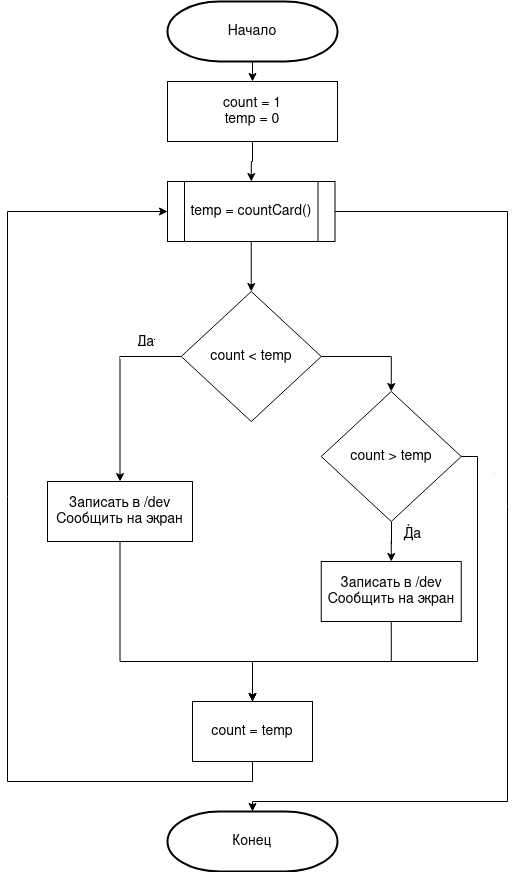
\includegraphics[,scale=0.6]{./img/b.png}
		\caption{Алгоритм пользовательской программы.}  
		\label{img:b}
\end{figure}

count --- начальное количество звуковых устройств;

temp --- текущее количество звуковых устройств;

/dev --- специальный файл, котороыйт обеспечивает протокол взаимодейсвтия пользовательской программы с модулем ядра.
\newpage
\subsection{Алгоритм управления индикатором}
Алгоритм управления индикаторм при получении сообщения

\captionsetup{justification=centering,singlelinecheck=off}
\begin{figure}[h!]
	\centering
		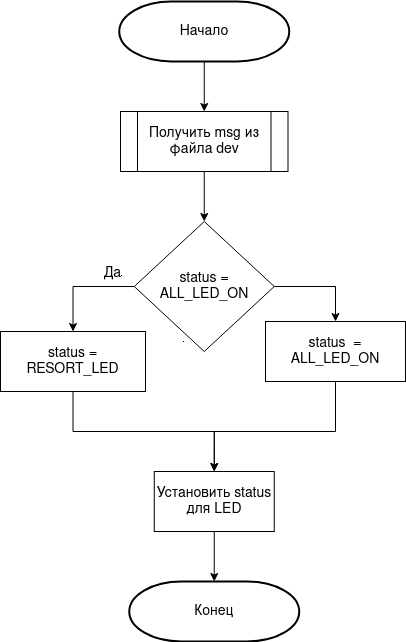
\includegraphics[,scale=0.6]{./img/c.png}
		\caption{Алгоритм управления индикаторм.}  
		\label{img:b}
\end{figure}